\cotefile{156-4}\scanpage{34}\mspage{33}
% @opening
sous-contrée ; \unsure{Idem} Ce terme est impropre. À moins de réserver le nom de ``contrée'' à \deleted{\uline{tout}} \inserted{\unsure{plus ou moins}} systèmes $(\unsure{\mathcal M|M},\ll,\unsure{\mathcal R|\mathcal Q}_{M})$. Je vais quand $=$ \unsure{réénoncer|r'énoncer} quelques axiomes, \unsure{potentiellement} cruciaux
% @cont1

\uline{Cont} \uuline{1} La relation ``$X\leq Y$'' ($\Longleftrightarrow X\ll Y$ et $X$ comp. $Y$) est une relation d'ordre
% @m1
% slanted
\margin{\uline{\unsure{Cont} 2} Si $X,Y$ sont compatibles, et $X'\leq X$, $Y'\leq Y$ alors $X',Y'$ compatibles}
% @fig2

\deleted{\unsure{Cont 2}} \inserted{\textcircled{\scriptsize Fig 2}} \deleted{\unsure{Toute}} Si $F\in\unsure{\mathcal F|\mathscr F}$, deux éléments \inserted{$X,Y$} de $F$ sont compatibles, et $F$ est une partie \uline{fermée} de l'ens $M(\unsure{\leq|\ll})$.
% @fig3

\deleted{\unsure{Cont 3|Cont 4}} \inserted{\textcircled{\scriptsize Fig 3}} Si $F$ \deleted{et $G$ sont deux} \inserted{est une} figure, \unsure{tte} partie $F'$ de $F$ qui est fermée, est une figure (appelée \uuline{sous-figure}).
% @m2
% slanted
\margin{\uline{NB} Si \deleted{\unsure{$F,G$}} $F',F$ sont des figures telles que $F'\subset F$, alors $F'$ est fermée dans $F$, \unsure{à cause} de Fig 1}
% @empty
% The text enclosed by the long contour is also the conclusion of the lower Cor.
\figure{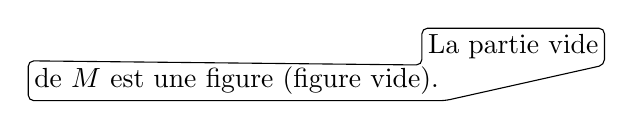
\begin{tikzpicture}[remember picture]
\node[anchor=south west,inner sep=2pt] (emptystart) at (5.0,.20) {La partie vide};
\node[anchor=west,inner sep=2pt] (emptyrest) at (0,0) {de $M$ est une figure (\uuline{figure vide}).};
\draw[rounded corners=2pt] (emptyrest.west) -- (emptyrest.north west) -- (emptystart.south west) -- (emptystart.north west) -- (emptystart.north east) -- (emptystart.south east) -- (emptyrest.south east) -- (emptyrest.south west) -- cycle;
\end{tikzpicture}}
% @fig1

\deleted{\unsure{Cont 3|Cont 4}} \inserted{\textcircled{\scriptsize Fig 1}} Si $X\in M$, l'ens \inserted{$F_{X}=M_{\leq X}$} des \unsure{$Y\in X$} \deleted{tels} \deleted{\unsure{que}} que \unsure{$Y\leq X$} est une figure, qu'on appelle la ``\uuline{figure élémentaire}'' \unsure{définie} par \uline{la} multiplicité $X$.
% @cor

\uline{Cor}. \inserted{(de \unsure{Cont} 2 et \unsure{Cont} 4)} Si $M\neq\varnothing$, \tikz[remember picture,baseline]{\coordinate (corend) at (0,.15); \draw[overlay,->] (emptyrest.west) .. controls +(-1.2,-1.6) and +(-.4,-.8) .. (corend);}
% @nb

\uline{NB} Si $M=\varnothing$, \deleted{Si $M=\varnothing$} l'axiome \uline{Fig \unsure{3|4}} devient vide -- on le remplace par \unsure{:} \deleted{la partie} \deleted{la \unsure{partie vide de|partie vide est} $M$} la seule partie de $M$ (savoir la partie vide) est une figure.
% @cancelled

\deleted{\uline{Cor} (de \uline{Fig 1} et \deleted{\unsure{la}} \uline{Fig 2}) Si \deleted{\unsure{$X$}}, $Y,Z$ sont tels que \unsure{$Y,Z$}$\ll X$, et si $Y,Z$ \unsure{st} comp. à $X$, alors \unsure{sont entre eux}}
